04\chapter{Evaluation of Typical Forecasting Tasks}\label{ch:eval_of_typ} 
\color[red]{Thoughts on this chapter:
\begin{itemize}
    \item How much detail do we need? So far, most technical details are avoided, meaning also that probably, additional sources have to be used to set up an evaluation framework. I think this is fine for this document and it would clearly be too extensive to cover every single aspect in detail.
    \item It could be worth to go through a complete evaluation exercise of a simple continuous and/or binary forecast task. An example could probably show much simpler what we mean in the different parts here but the problem is that it could become quite lengthy if we want to cover multiple interesting features.
\end{itemize}

}

The characteristics of a “typical forecasting task” is defined in this context as forecasts generated to fulfill operational obligations in electric system operation  or trading and balancing of renewable energy and in particular wind power in power markets. There are certainly many other tasks and applications of weather and power forecasts in the power industry that can benefit of the following recommendations as well. However, the target application for the following recommendations are focusing on the evaluation of these tasks in particular. 
These recommendations will be extended to the evaluation of trials and operational forecasts in Chapters \ref{ch:eval_of_trials} and \ref{ch:eval_of_oper}, respectively.

\color{red} 
Perhaps introduce continuous power forecasts and binary forecasts as typical tasks

One may quantify desirable qualities by considering a range of of dichotomous (yes/no) events such as high-speed shut-down or ramps. A forecast might imply that "yes, a large ramp will happen" and trigger the user to take action, but the ability of a forecasting system to make such predictions is not clear from the average error metrics. Therefore, one should employ a quantitative verification approach to assess this ability by analyzing the number of correct positive, false positive, correct negative and false negative predictions of particular events [Hamill2006].
\color{black}

 
\section{General Considerations}
\subsection{Selection of Evaluation Metric}
When evaluating a forecasts on has to select one or several evaluation methods or metrics to measure and compare the forecast performance. 
Unfortunately, there does not exist one single best metric and it highly depends on the intended application of the forecast user, which metric gives the most meaningful results.
E.g., if the user has to pay a penalty for forecast errors that is proportional to the squared error, a mean squared error metric is well suited, while if the penalty is proportional to the absolute error a mean absolute error should be used. Similarly, mean squared or absolute errors do not reveal any information about the suitability of a forecast to predict specific events such as high wind shutdown or ramps.

Therefore, it is crucial to select the evaluation metrics carefully and base it on the loss function of user. If one forecast is used for different applications with different cost functions, a set of metrics can be derived and weighted based on their importance.
More details on how to develop cost functions and evaluation matrices can be found in \ref{sec:costfunc}

\subsection{Uncertainty of Evaluation Results}\label{sec:uncertainty}

Evaluation results are, just as forecasts themselves, always subject to a certain degree of uncertainty. That means, evaluation results will in general depend on the data set used to derive them and will be different for different data sets.  
The degree of uncertainty is variable and mostly depends on the size of the evaluation data set, meaning that if an evaluation data set is large, the results can be trusted more than for small data sets.
Since the data set size is usually limited by the benchmark or trial design, it is important for basing decisions on these results, to be aware of and measure this uncertainty.
Section~\ref{sec:significance} provides more details on bootstrap resampling and parametric testing to estimate the uncertainty or significance of evaluation results.

%There are difference methodologies to do this. A relatively simple methodology that is easy to establish are error frequency distributions, also called probability density functions, in form of curves, bars or tables. By sorting the errors in ranges (bins), it is possible to  
%\begin{itemize}
%    \item analyze the distribution or types of errors 
%    \item characterize errors and identify random high outliers  
%\end{itemize}
%The shape of error distributions provide an indication of forecast performance and can be related to the problem a forecast is supposed to solve. Average error metrics can too easily provide misleading performance results for a forecast, especially in short test periods. The interpretation of frequency distributions are explained in the development of a forecast performance framework section \ref{sec:freqdist}.  

%While error frequency distributions can provide a glance of the variations in the forecast errors, resampling (bootstrap) methods or parametric test frameworks such as the one proposed by \citet{Diebold1995} can give more insight on the significance of evaluation results and should be applied in all evaluation tasks. More details on these approaches can be found in \ref{sec:testing}.



%Another way to identify uncertainty in results is by using box plots, or also known as Box-and-Whiskers plots .     

%Diebold [1995] proposed a parametric test framework to estimate the significance of score differences. Alternatively, non-parametric bootstrapping methods can be applied [Efron, 1981]. 

%Both parametric testing and bootstrapping operate on the individual error measures (e.g., the squared or absolute error before averaging) and are thus easy to implement or even readily available in various software packages. Easy to understand guidelines on how to interpret the results will be given in the IEA Recommended Practice documents. 

 

\section{Developing an Evaluation framework}\label{sec:evaluation_framework}
For every evaluation task, benchmark or trial an evaluation framework has to be defined. In the case of a trial this framework should ideally be defined before the start of the trial and be communicated to the participants. This is important for a fair and transparent trial and a well designed evaluation framework ultimately ensures that the forecast users receive forecast solutions that are tailored to their needs.

This section introduces the most important parts of an evaluation framework.

\subsection{Time Definitions in Forecasts}
Time is an important aspect of forecasting and it is crucial to clearly define the delivery and forecast times.
\begin{itemize}
    \item Initialization time: Is the time the forecast computation is started. Only data before this time can be used as input to the forecast model.
    \item Forecast delivery time: Is the time the forecast is provided and can be used. Because of computation and transfer times the forecast delivery time can differ from the initialization time.
    \item Look ahead time or lead-time: Is the time between initialization time and the forecast time.
    \item Forecast time: Is the time to be predicted.
    \item Forecast horizon: the largest look ahead time available.
\end{itemize}

\subsection{Evaluation data set}
Before any evaluation task it is important to prepare the evaluation data set appropriately.
An evaluation data set is a set of forecasts for different dates/times and the corresponding observations, typically given stored in a table with one row for each date and the observations and forecasts as columns. 
If multiple forecast models are to be compared, there can be several forecast columns and for a fair comparison it is important to disregard all rows with at least one missing entry. 
Else, a forecast model that avoids to predict difficult forecast situations (e.g., forecasts in an uncertain weather situation) will receive better scores than forecasts that are always available.

It is also important to be aware of other differences in the forecast task, such as lead times, time of day, seasons etc. 
It is of course possible to derive errors for all of these combined, and if e.g., the cost of forecast errors for different lead times is equal, a combined measurement can also be appropriate. 
However, clearly some details of the forecast performance are hided in such an approach and e.g., if many lead times are combined together, the error measure will be dominated by the usually larger errors of longer lead times.


\subsection{Basic analyses of forecasts and forecast errors}
Prior to any other analysis the forecasts should be checked for consistency and analyzing the forecast error can provide a first glance of the forecast quality and help to establish cost functions or evaluation matrices.
This section presents some basic approaches to analyze forecasts and forecast errors.

\subsubsection{Basic verification methods}
Forecast verification is the practice of comparing forecasts to observations. While this includes quantitative approaches, such as the metrics discussed above, it may also include qualitative verification of the forecast model and its outputs. Forecast verification serves to monitor forecast quality, compare the quality of different forecasting systems and also as a first step towards forecast improvement. 

The simplest form of forecast verification for continuous forecasts is visual inspection with e.g., time series plots or histograms. Does the forecast look right? Does it have the same properties as measurements of the target variable? For instance, a wind power forecasting tool should exhibit the behavior associated with the wind turbine power curve: cut-in, below-rated and rated power, and so on. It may also be desirable that forecasts are consistent across space and time, if receiving forecasts for multiple wind farms in a portfolio for instance. 

Another simple but informative visualization is the scatter plot of predicted versus measured wind speeds, which shows a cloud of simultaneous pairs of measurements and forecasts. The narrower the cloud along the identity line, the better they match each other. Systematic errors result in a point cloud that deviates from the diagonal. Periods of constant measurement are visible as straight lines which will reach outside the dense cloud of points.  

\color[red]{Example time series and scatter plot}


Visualization plays a large role in qualitative verification and there are many other possible plot types that can help in analyzing the quality of a forecast system.
E.g., errors versus forecast power can rapidly identify periods of poor performance or some types of systematic error.

For the forecast of dichotomous (yes/no) events, such as  high-speed shut-down or ramps, a typical analysis tool are contingency tables that summarize the hits and misses of these forecasts and can answer questions like ``What fraction of ramp events were correctly forecast?'' and ``What was the accuracy of the forecast relative to random chance?''.

\color[red]{Example contingency table}

This kind of verification is often useful at the preliminary stage in a more detailed verification exercise. This "quick glance" approach is especially useful if there aren't many forecasts to evaluate or very limited time. This approach is subjective and so should be complemented by objective measures. 





%Such an analysis can answer questions like ``What fraction of ramp events were correctly forecast?'' and ``What was the accuracy of the forecast relative to random chance?''. 

%Verification can be very useful when comparing forecasts that aim to support specific decisions, such as managing ramps in the example above. However, care must be taken when interpreting quantitative results. Only considering the proportion of events that were successfully predicted, or calculating error metrics only during specific events can produce misleading results. This is known as the `forecaster's dilemma' [Lerch,2017]. 

%Put simply, one can successfully predict every extreme by always forecasting its occurrence. If the forecast is only evaluated when the event occurs, this would appear to be a perfect forecast!

\subsubsection{Analysis of forecast errors}
Forecast errors (here defined as forecast minus observation) in wind power forecasting are almost inevitable but should be as close to zero as possible. 
Direct analysis of these errors can provide a lot of insight into the forecast performance and in which situations the forecasts excel and when they fail.

Frequency distribution of errors or often also referred to as density functions or probability density functions are established by sorting errors and visualizing their distribution as e.g.,  
\begin{itemize}
    \item (probability) density curve 
    \item histogram (frequency bars)  
    \item box plot
\end{itemize}
All of these plotting types show the same basic information but with different degrees of detail.
While density curves estimate the full probability density function of forecast errors, histograms show the frequency of a number of error categories and box plots condense these informations into several quantiles.
Errors of a well calibrated forecast model should always be scattered around zero and a frequency distribution that has a center shifted from zero indicates a systematic error.
For power forecasts one will often see positively skewed error distributions, which are often caused by forecasts close to zero not being able to have large negative errors.

\subsubsection{Example of a box and wiskers plot}\label{subsec:boxplot}

One example of using the box-and-wiskers plot to analyise forecast performance is to visualize the error spread of different forecasts of different forecast time horizons. In that way, the spread of forecast performance in each hour of the day-ahead horizon can be visualized. It also shows how some forecasts in some hours show very low errors compared to the average error in that hour, as well as occasionally very high errors. Figure \ref{fig:boxplot} shows the principle of a box and whiskers plot. In section \ref{sec:significanceTestExample}, a use case for the application of box plots is demonstrated to verify significance of results. 

\begin{figure}[h!]
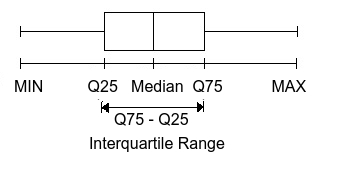
\includegraphics[width=0.9\textwidth]{figures/box-wiskers-plot.jpg}
\caption{Principle of a box-and wiskers plot. The plot displays the five-number summary of a set of data, which is the minimum, first quartile, median, third quartile, and maximum. In a box plot, a box from the first quartile to the third quartile is drawn to indicate the interquartile range. A vertical line goes through the box at the median.}
\label{fig:boxplot}
\end{figure}



\subsubsection{Examples of the use of histograms}\label{subsec:historgram}

Histograms allow one to quantify the frequency of occurrence of errors below or above a certain level and mentioned two important conclusions that can be drawn from histograms and that such statistics can be summarized by plotting the percentage of time that errors are within a given margin [\cite{madsen2005}]:\\
\begin{itemize}
    \item Robustness
    \item Large Errors
\end{itemize}

Madsen et al. \cite{madsen2005} shows an example in how such histograms can be interpreted. In their example, they could directly read out that e.g. a 1 hour-ahead prediction contained errors less than 7.5\% of the available capacity in 68\% of the time, while a 24 hour-ahead prediction may show errors of that size only in 24\% of the time. For large errors, they read out of the histogram that the same 1 hour-ahead prediction's largest errors were 17.5\% of available capacity in only 3\% of the time.

Figure  \ref{fig:figure2} provides two example histograms with typical frequency distribution of errors for a 2-hour forecast horizon (left) and a day-ahead horizon (right) as described in \cite{madsen2005}.

\begin{figure}[h]
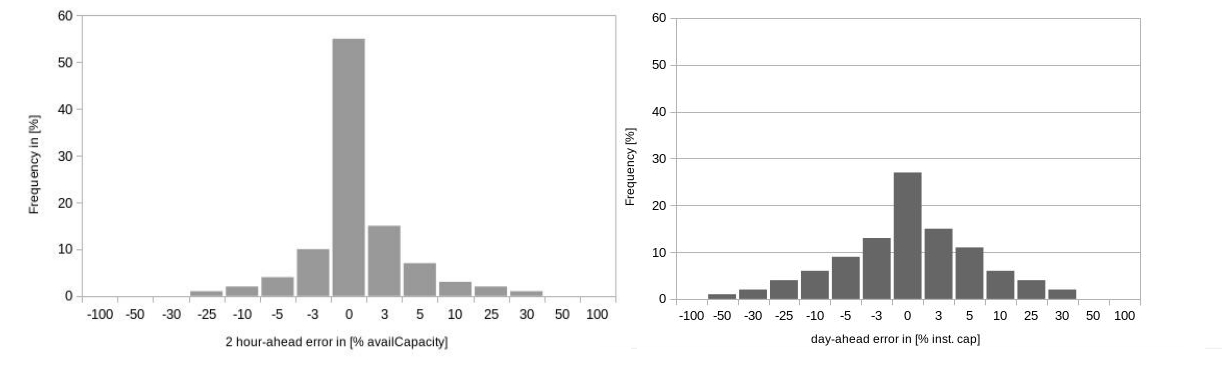
\includegraphics[width=0.9\textwidth]{figures/freq2plots.jpg}
\caption{Examples of two histograms showing typical frequency distribution of errors for a 2-hour forecast horizon (left) and a day-ahead horizon (right). }
\label{fig:freqency}
\end{figure}


\subsection{Recommendation}

Due to the complexity of the task and the fact that no one forecast user's objectives are the same, the following recommeendation for best practice focuses on providing a framework of tasks in order to establish structured procedures for the evaluation and verification of forecasts. Dependent on the size of the forecasting system and the imprtance in the overall business processes, the structure may be shortened and adopted to fit purpose.
Best practice here is defined to follwoing a procedure, where the evaluation and verification reflects the importance of a forecasts in it's role in the busniess processes and provides incentives for the forecast service provider to generate forecasts that fit the outlined and verified purpose. 

The minimum requirement when establishing such an evaluation framework contains the following set of procedures: 
\begin{enumerate}
    \item \textbf{Definition of the forecast framework} \\
        It is important to define exactly what the forecasts are used for, which time frames are used for which applications and set a ranking on importance.

    \item \textbf{Base performance evaluation on a clearly defined set of forecasts} \\
     The base performace should contain average error metrics in order to monitor an overall performance level.
        \begin{itemize}
            \item time frame:  minimum 3 months, ideally 1 year
            \item average error metrics: nMAE, nRMSE, BIAS
        \end{itemize}
    
    \item \textbf{Quality assessment of  the  considered  data}  \\
        The detection  of  missing  or  erroneous  data and a clear strategy how to deal with such missing data needs to be made at the outset of any project and verification period to ensure that verification and forecasting is fair and transparent.
    
    \item \textbf{Specific Performance evaluation on a set of error metrics} \\ 
       \begin{itemize}
            \item Visual Inspection
            \item use of more specific metrics: SDE, SDBIAS, StDev, VAR, CORR
            \item Use of histogram or boxplot for evaluation of outliers
            \item use of contingency tables for specific event analysis
            \item Use of improvement scores for comparisons
       \end{itemize}
    
\end{enumerate}

Note, details on the framework and evaluation metrics can be found in  \cite{madsen2005} and \cite{messner}, specific metrics and explanation of metrics can be found in \cite{jensen}, \citet{zhang2015} for deterministic forecasts inclusive solar forecasting and for probabilistic forecast mtrics in \cite{anemosplus}. Significant tests can be found e.g. in \cite{vogt2018}.



%The frequency distribution from one year of 15 minute mean values of a wind speed shall be a smooth curve with decreasing probability of high wind speeds. A temporary instrument fault will be visible as a skewness of the curve. We compare frequency distributions of the ensemble mean forecast against measurements.  

%Positive and negative phase errors between forecast and measured data tend to cancel each other out over a long enough period. Therefore, one should expect high similarity between two independent time series of the same physical variable.  

% Figure shows the principles of historgrams and the correcsponding error distribution curve.  

 

%In many real-time examples the error distribution curve looks slightly different, because error ranges are chosen uneven or can also sometimes be used as absolute error, rather than making a distrinction between positive (overprediction) and negative (under-prediction) errors. Nevertheless, these principles are always the same and provide the possibility to chategorise errors and incentivice performance, where it is most important for the operations.  

 



 

%\subsubsection{Box and Wisker Plots }

 

 

%Case 1: Comparoison of forecasts at different time horizons 



%The example in  Figure shows the spread in MAPE (mean absolute error as percentage of nominal power) of 5 forecasts of different day-ahead time periods (each column, starting with ST=short-term, DA=day-ahead, x=time of day) at two different sites (left and right). The distribution within each time period is shown for the MAPE error of 5 forecasts. 

%[Text Box] 

%The important information to take away from such an analysis is how much spread there is in the performance of the tested forecasts and whether this is so  over the entire forecast horizon. In short tests, random outliers that have large impact on the result can be easily detected and evaluated, whether or not such an error is significant for the overall performance of a forecast. For example, if a large errror for one forecasts at one site and 1 specific period within the forecast horizon cannot be detected at other sites, such an outlier may be random and marked as such in the overall evaluation of a forecast performance. In short tests such one outlier can give the impression of a bad forecast performance without objective reason.  

%This is where the subjective evaluation takes place with objective means. It is a way to secure fairness and to create representative and repeatable results.  

\subsection{Quantitative Evaluation methods }
Quantitative evaluation methods are usually the core of the evaluation framework since they allow to objectively rank different forecast models.
Typical choices of quantitative metrics are the (root) mean squared error, the mean absolute error or the quantile score (see \cite{Messner2018} for details) for continuous forecasts and various quantities derived from contingency tables for forecasts of binary forecasts.

As emphasized in Section \ref{sec:costfunc}, the selection of metrics should be adjusted to the cost function of the forecast user and if a forecast is intended to be used for multiple applications, different basic metrics should be applied and merged into a weighted sum. 
E.g., in energy trading, forecast errors are usually penalized proportional to their absolute value so that mean absolute errors are well suited. 


\subsection{Significance of evaluation results} 
%moved to 02_evaluation_uncertainty
As already noted in Section \ref{sec:uncertainty}, evaluation results are always subject to uncertainty. Thus, quantifying this uncertainty is important for decision making. E.g., if a number of forecast models are evaluated with a certain metric but their differences are much smaller than their uncertainty, the meaning of their ranking is actually very limited and should not be used for important decisions.

The variation or uncertainty of evaluation results mainly stems from their dependence on the evaluation data set and results so that results can vary for different data sets.
The simplest approach to estimate this variation would be to repeat the evaluation task several times on different data sets. However, since evaluation data sets are usually very limited, this is not a feasible approach. 
As a simple method to simulate different data sets, bootstrap resampling can be used. Therefore, a set of the same length as the data set is drawn from the data set with replacement and the evaluation results are derived on this set. By repeating this e.g., 100 times, 100 different evaluation results become available and their range can be seen as the evaluation uncertainty.

Alternatively, parametric testing can also provide information on the significance of evaluation results. 
Typically two sample paired t-tests applied on the sets of error measures for each event provide a good estimate of the result significance. 
\citet{Diebold1995} proposed a variation of this t-test to account for temporal correlations in the data and can therefore provide a more accurate significance quantification.
 
 
\subsubsection{Example of a Significance Test and Best Practice} \label{sec:significanceTestExample}  % NOW in 05_best_practice \ref{sec:significanceexample}


As dicussed above, forecasts and their quality can vary greatly, depending on the model or input data used. Forecast vendors, customers and researchers are therefore often confronted with the question which forecast to choose. 
In the following example, a typical situation is presented and outlined starting with the overall considerations, followed by the choice of metrics and test on significance on the results. 

\emph{Initial Considerations}
A forecasting model that can take various inputs, such as online measurements in an autoregressive manner, weather forecasts or other predictive features, generates power forecasts, which estimate the future electricity production. In order to decide which model is most suitable, it is necessary to evaluate its quality by comparing the forecast against power measurements. Typically, the errors of a separate test data are compared against each other in order to then decide in favor of one of the models. Which error measure is chosen should be individually adjusted to the corresponding application.

The evaluation should be performed strictly on test data that were not used to calibrate the respective model.  Otherwise it can easily happen that models are favored, which have adapted too much to the training data without being able to generalize for future unknown situations. If several models are compared, they should also have been jointly trained on data that does not originate from the test set. 

In the case of wind power forecasts, it is furthermore essential to select the test data from a continuous period. The data cannot be considered temporally independent. If one were to randomly assign individual samples to a training and a test set, one would assign both sets to random samples that share a large part of the information. As a result, preference would also be given to models that are overadapted to the training data.

In addition to the error measure, other aspects can also play a role. For example, one is faced with the question of whether an established model should be replaced. For several reasons it may seem attractive not to replace it even though another one shows a smaller error. For instance, because confidence in the model functionality has been built up, or because a change in the model requires additional effort. Such or similar cases make it necessary to examine the significance of the estimated error values. The critical question behind this is whether the extent of the test data considered is sufficient to form the basis for a decision. 

\emph{Evaluation of Significance}
One way to evaluate the significance of the error values is to evaluate the distribution of the error measures of a model across different locations. In the following, the relevant aspects of the results of the study in [Vogt2018] are summarized. It compared different machine learning models for weather forecasting and real-time measurement based forecasting. The box plot shown in Figure \ref{fig:significance} shows the distribution of the error measures of 29 wind farms in northern Germany. The error measure used here is the root mean square error (RMSE) which is applied to nominal power normalized time series.
The individual boxes represent the error distribution of one of the six models used.  The triangular markers indicate the confidence range of the median. If these ranges do not overlap for two models, the medians are different under normal distribution assumption to a 5\% significance level. This corresponds to a visual representation of a t-test. 


\begin{figure}[h!]
 \begin{subfigure}
  \centering
  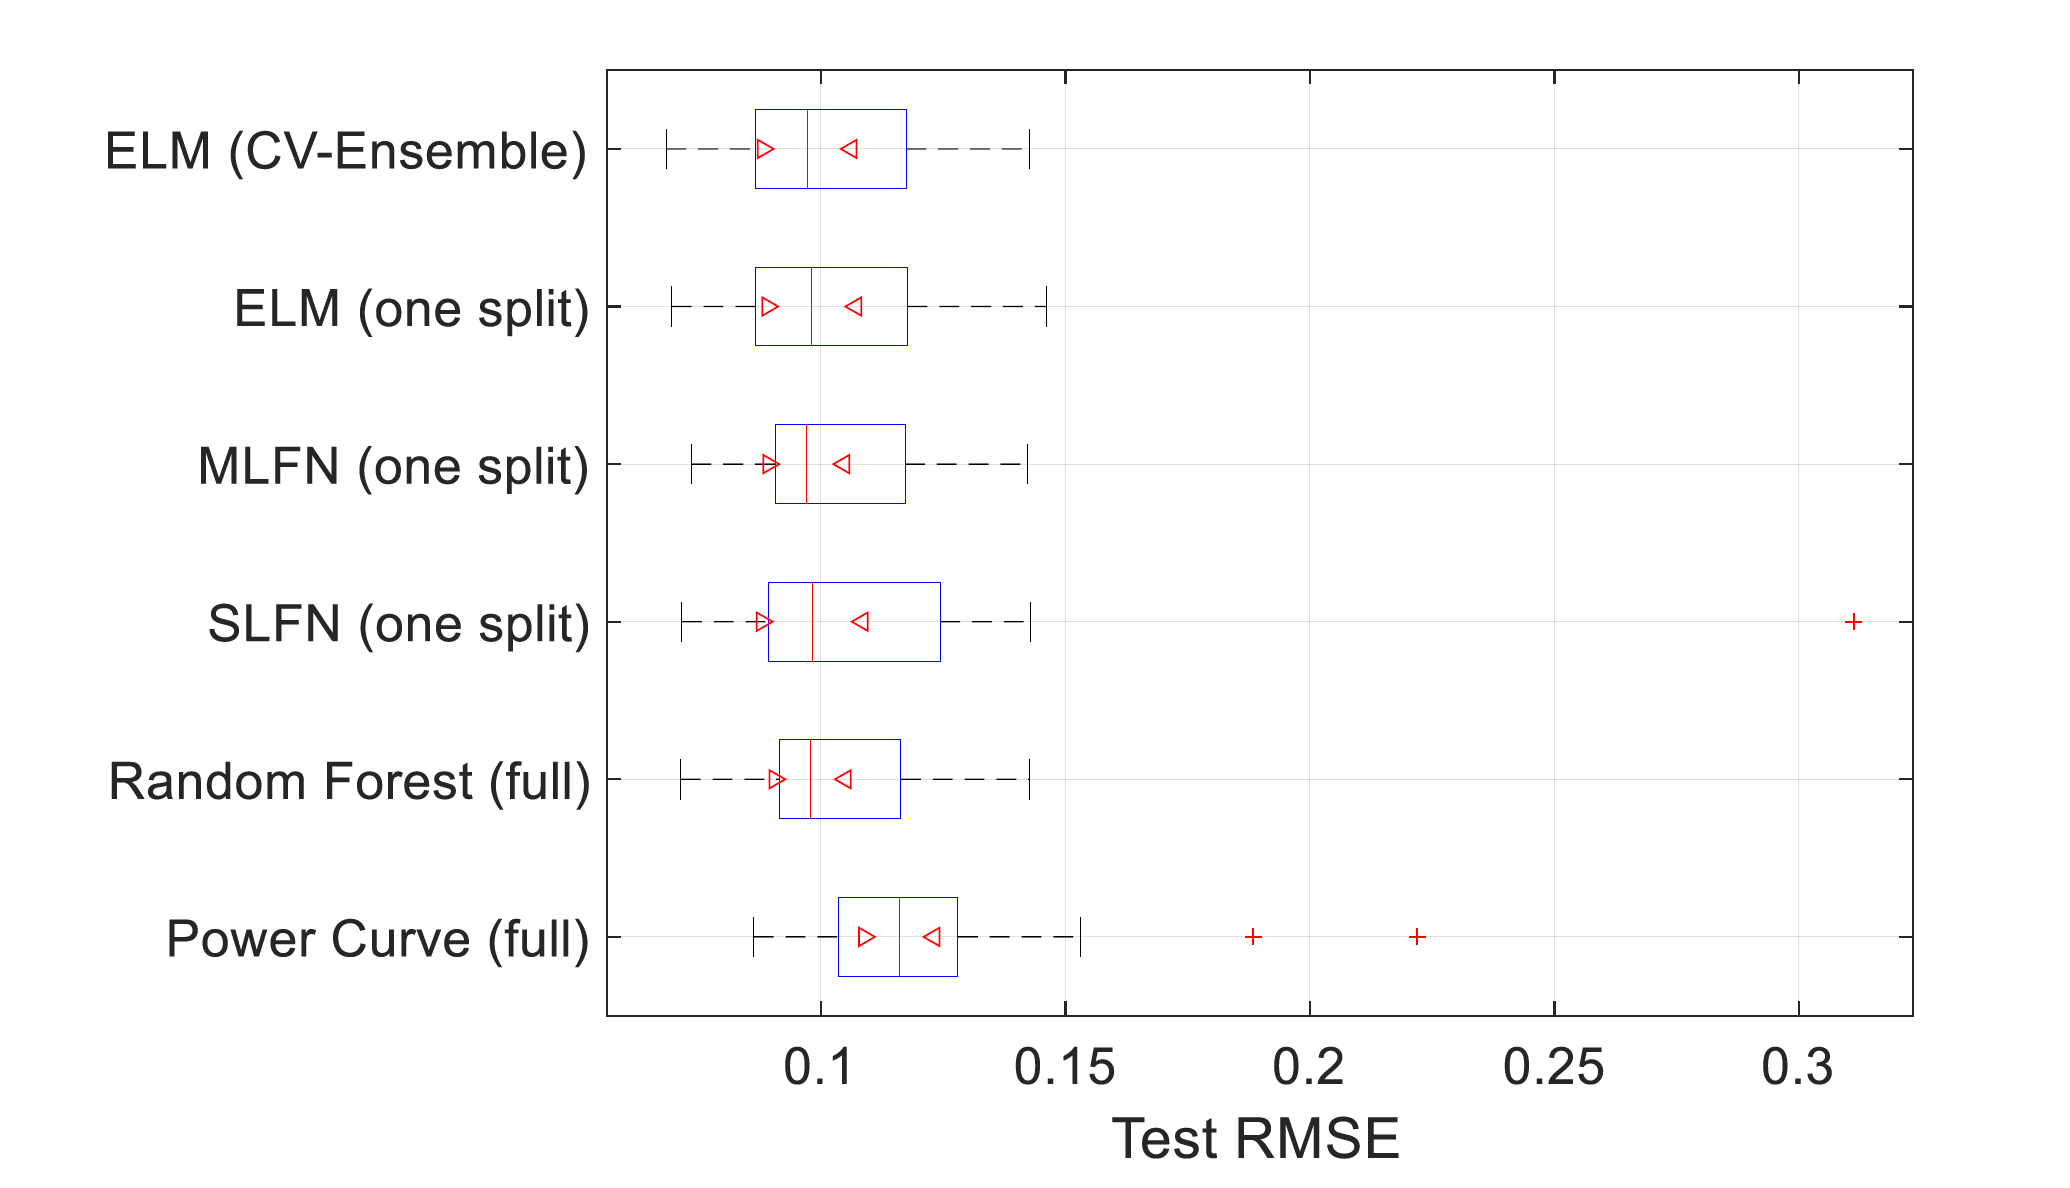
\includegraphics[width=0.48\textwidth]{figures/significance1.png}
 \end{subfigure}
\begin{subfigure}
 \centering
 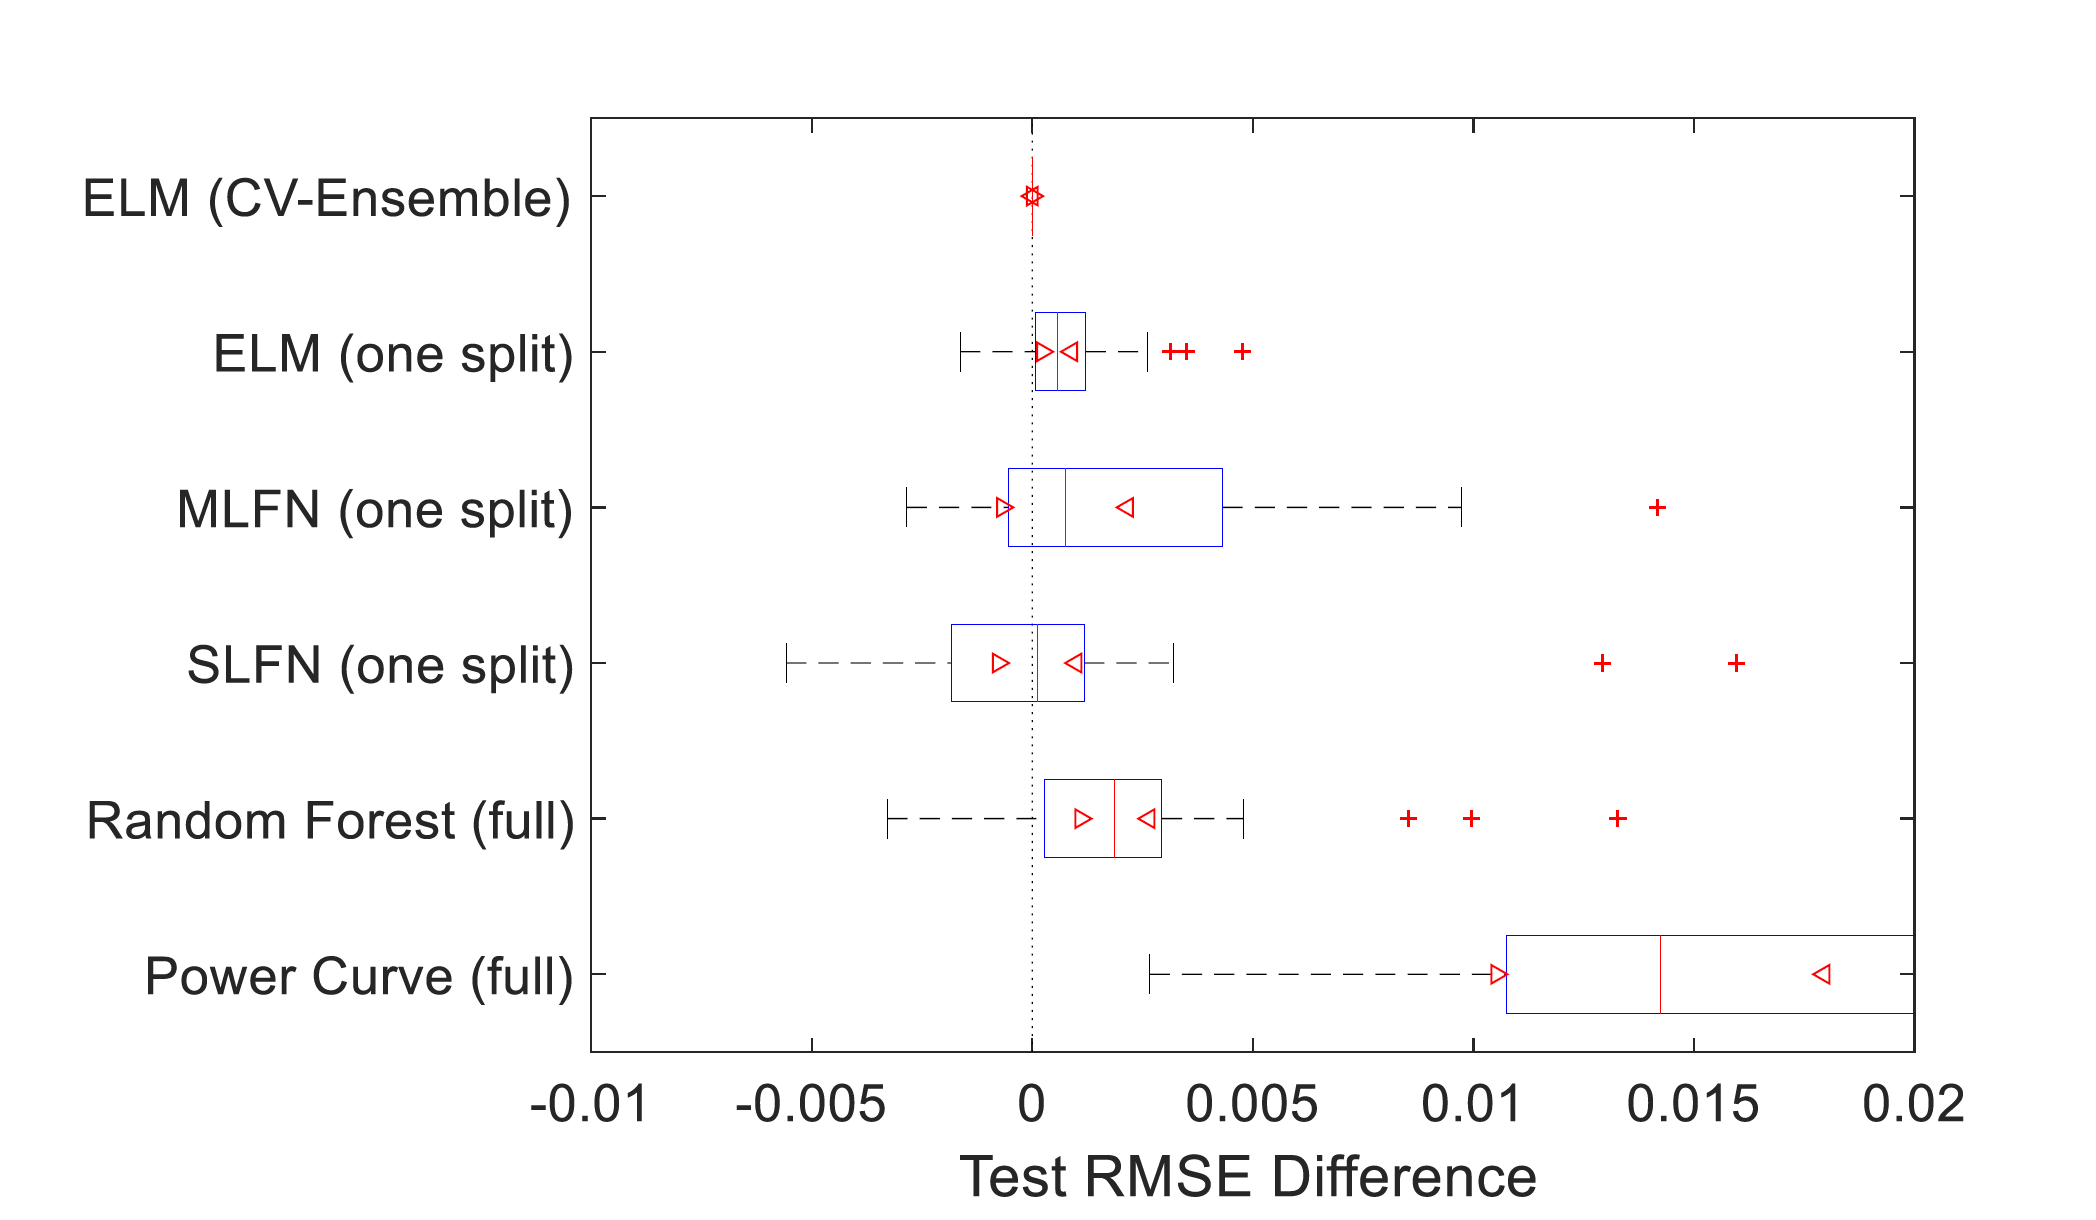
\includegraphics[width=0.48\textwidth]{figures/significance2.png}
\end{subfigure}
\caption{RMSE distribution for six different forecasting models forecastng for 29 wind farms in the North of Germany (left figure). Pairwise differences RMSE for each single model in comparison to the wind farm RMSE of the reference model ELM (CV-Ensemble) \cite{vogt2018} (right figure). }
\label{fig:significance}
\end{figure}

Figure \ref{fig:significance} (left) shows, that only the power curve model has a significantly higher RMSE. All others cannot be clearly distinguished. The reason for this can be found in the broad distribution. This can be explained to a greater extent by the different local properties, such as the number of turbines per wind farm or the local orography. When considering the paired differences, local influences can be partially eliminated. \\

Figure \ref{fig:significance} (right) shows the distribution of the difference between a model and a reference model (ELM (CV-Ensemble)) across all 29 wind farms. If the distribution of a model is significantly in the positive range, it can be assumed that the reference model is significantly better. Thanks to these pairwise differences, it can now be established that two other models have a significantly worse result.  



\section{Developing a cost function or Evaluation Matrix  }\label{sec:costfunc}

\subsection{Cost functions }
%The resulting cost functions should then be defined by the forecast users expectations and requirements for the forecast. Only then, it is possible to also setup a meaningful verification and comparison.  
It has already been mentioned at several places in this document but cannot be emphasized enough that the forecasts should always be measured by metrics that reflect the cost function of the forecast user.
Unfortunately, such cost functions can quickly become quite complicated, when one forecast system is intended to be used for a range of applications. 
For example, it is not possible to establish a single function that could verify a day-ahead average forecast performance together with a forecast of ramps. Such two products have different targets and hence different methods are used to generate such forecasts. Therefore, any forecast user needs to be clear about the usage of a forecast product and the associated performance target. A ramp forecast may be evaluated with a contingency metric, while a day-ahead forecast will be verified with RMSE or MAPE. In the same way there could be criteria (cost functions) that weigh large errors much higher than small errors due to reserve requirements, such that two forecasts of similar average performance may be different in their error pattern.  
The only way to ensure the performance metric fits to the performance requirements is by developing a framework of metrics and an evaluation of ranges of errors and give them weights in accordance to their costs or importance.  

Furthermore, it is not always very clear, how the forecasts enter the final decision making process since they are often used as one of many inputs for decision makers.
Thus it is important for the forecast users to evaluate their decision making processes and at least come up with an estimate of how the forecasts effect the final decision making and how much an error in these forecasts will translate into financial losses.

\subsection{Evaluation Matrix  (Corinna)
